\documentclass[12pt, a4paper]{article}
\usepackage[T1]{fontenc}
\usepackage[utf8]{inputenc}
\usepackage{lmodern}

\usepackage[german]{babel}
\usepackage{amsmath}
\usepackage{amsfonts}
\usepackage{amssymb}
\usepackage{graphicx}
\usepackage{hyperref}

\usepackage{listings}
\usepackage{xcolor}

% Define code listing style for Python
\lstdefinestyle{mystyle}{
	language=Python,
	basicstyle=\ttfamily,
	keywordstyle=\color{blue},
	commentstyle=\color{green},
	stringstyle=\color{purple},
	numbers=left,
	numberstyle=\tiny\color{gray},
	breaklines=true,
	frame=single,
	showspaces=false, % Zeige Leerzeichen
	showstringspaces=false, % Zeige nur Leerzeichen in Zeichenketten
}



\title{Natural Language Processing Projekt: \\ Question Answering Systeme}
\author{M.Sc. Onur Yilmaz}
\date{\today}
\newcommand{\supervisor}{Betreuer: Prof. Dr. Gawron}

\begin{document}
	
	\maketitle
	
	\begin{center}
		\supervisor
	\end{center}

\thispagestyle{empty}
\newpage
\tableofcontents
\thispagestyle{empty}
\newpage

\section*{Einleitung}
In einer Ära, in der leistungsstarke Sprachmodelle wie GPT-3 die Grenzen der natürlichen Sprachverarbeitung neu definieren, gewinnt das Gebiet der Frage-Antwort-Systeme (Q\&A-Systeme) eine noch größere Bedeutung. Diese Modelle, die auf bahnbrechenden Fortschritten in der künstlichen Intelligenz basieren, ermöglichen es, menschliche Sprache in nie dagewesener Weise zu verstehen und zu generieren. Diese Ausarbeitung taucht tief in die Welt der Q\&A-Systeme ein, die auf solchen fortschrittlichen Sprachmodellen aufbauen. 
\\ \\
Im ersten Teil liegt der Fokus auf dem Verständnis der Konzepte und Techniken im Bereich des Question Answering Systems. Dabei werden die Grundlagen und Herausforderungen dieses Feldes beleuchtet. 
\\ \\
Im zweiten Teil widmet sich die Ausarbeitung einem umfangreicheren Question-Answering Projekt, bei dem die praktische Umsetzung in den Mittelpunkt gerückt wird.





\newpage
\setcounter{page}{1}
\section{Hintergrund}
\subsection{Natural Language Processing}
Natural Language Processing (NLP) ist ein interdisziplinäres Feld, das an der Schnittstelle von Informatik, künstlicher Intelligenz und Linguistik angesiedelt ist. Ziel des NLP ist es, Computern die Fähigkeit zu verleihen, menschliche Sprache zu verstehen, zu interpretieren und zu generieren. Dies umfasst eine breite Palette von Aufgaben, darunter maschinelles Übersetzen, Sentimentanalyse, Textzusammenfassung, automatische Textklassifikation und mehr. In den letzten Jahren haben wir eine beispiellose Entwicklung im Bereich der NLP erlebt, die insbesondere durch den Einsatz von maschinellem Lernen und tiefen neuronalen Netzwerken vorangetrieben wurde.
\\ \\
Eine bedeutender Wegbereiter dieser Fortschritte ist die Plattform \textbf{Hugging Face}. Hugging Face hat es sich zur Aufgabe gemacht, die neuesten und leistungsstärksten NLP-Modelle der Welt zugänglich zu machen. Durch die Bereitstellung von vorgefertigten Modellen, Tokenizern und Trainingspipelines hat Hugging Face die Entwicklung von NLP-Anwendungen erheblich vereinfacht und beschleunigt. Modelle wie GPT-3, BERT und T5 haben die NLP-Community revolutioniert und bieten beeindruckende Fähigkeiten bei der Verarbeitung und Generierung von Text.
\subsection{Question Answering Systeme}
Question Answering (QA) Systeme sind spezialisierte Anwendungen von NLP, die darauf abzielen, präzise Antworten auf Fragen der Nutzer in natürlicher Sprache zu liefern. Diese Systeme können auf einer Vielzahl von Datenquellen basieren, einschließlich strukturierter Datenbanken, dem Internet oder spezifischen Textkorpora. QA-Systeme sind besonders nützlich für die Informationsgewinnung und können in verschiedenen Bereichen wie Kundenservice, Gesundheitswesen oder Bildung eingesetzt werden.

\subsubsection*{Aufbau eines Q\&A Systems}
Der Aufbau eines Q\&A Systems kann in mehrere Kernkomponenten unterteilt werden:
\begin{itemize}
	\item \textbf{Frageanalyse:} Hier wird die Benutzerfrage analysiert und verstanden. Dazu gehört die Identifikation des Fragetyps und das Extrahieren von Schlüsselbegriffen.
	\item \textbf{Dokumentenabruf:} In diesem Schritt werden relevante Dokumente oder Informationsquellen basierend auf der analysierten Frage abgerufen.
	\item \textbf{Antwortgenerierung:} Nachdem relevante Informationen abgerufen wurden, wird eine Antwort generiert. Dies kann durch Extraktion von Informationen aus den Texten oder durch Generieren von neuen Texten basierend auf den gefundenen Informationen erfolgen.
	\item \textbf{Antwortranking:} Schließlich werden die generierten Antworten bewertet und die beste Antwort wird dem Benutzer präsentiert.
\end{itemize}
\ \\
Jede dieser Komponenten stellt eigene Herausforderungen dar und es gibt verschiedene Ansätze und Technologien, um diese zu bewältigen.   \\  \\
\subsection{Einblick in die Funktionsweise eines QA Systems} \ \\
Um einen Einblick in die Funktionsweise eines Frage-Antwort-Systems (Q\&A) zu erhalten betrachten wir den \textbf{SQuAD 2.0}-Datensatz.
\\  \\
Der SQuAD 2.0-Datensatz (Stanford Question Answering Dataset 2.0) ist ein Datensatz für die Aufgabe des Question Answerings. Im Gegensatz zum ursprünglichen SQuAD-Datensatz enthält SQuAD 2.0 nicht nur Frage-Antwort-Paare, bei denen es eine eindeutige Antwort gibt, sondern auch solche, bei denen die Antwort unmöglich ist oder in den gegebenen Textpassagen nicht gefunden werden kann. Dies macht den Datensatz anspruchsvoller und realistischer.
\\
\begin{lstlisting}[style=mystyle, numbers = none]
from datasets import load_dataset

squad_v2_dataset = load_dataset('squad_v2')
\end{lstlisting}
\ \\
Mögliche Antworten auf einzelne Fragen sind in Form eines verschachtelten \textit{Dictionarys} gespeichert. Um hier uns einen besseren Überblick zu verschaffen, sehen wir uns das Ganze in einem DataFrame an:
\ \\
\begin{lstlisting}[style=mystyle, numbers = none]
import pandas as pd	

train_dataset = squad_v2_dataset['train']

df = pd.DataFrame(train_dataset)
df.head()
\end{lstlisting}
\begin{figure}[h!]
	\centering
	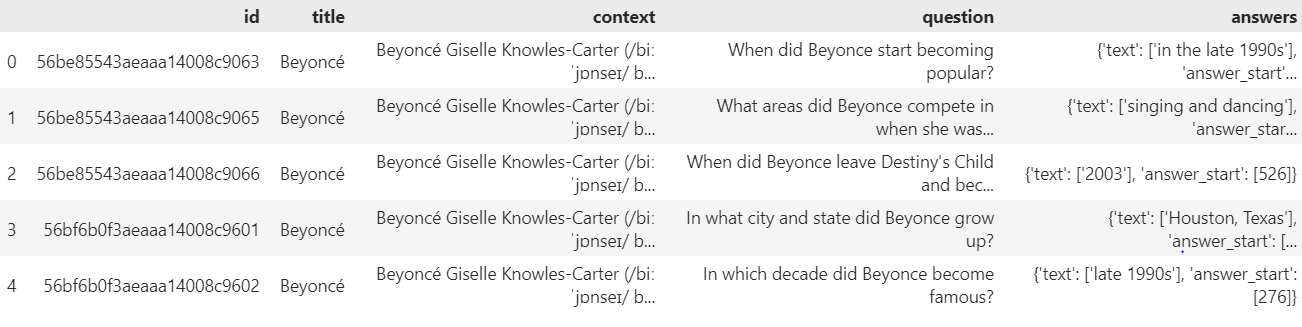
\includegraphics[width=1	\linewidth]{images/dataframe}
\end{figure}
\ \\
Nun wollen wir untersuchen, wie es mit den sog. \textbf{Transformer-Modellen} von \textbf{Hugging-Face} gelingt, gezielt Antworten aus einem Text zu extrahieren. Da es um Fragen geht, dessen Antworten in einem Datensatz identifiziert werden können, handelt es sich hierbei um ein sog. \textit{extraktives QA System}.
\\ \\
Auf der Hugging-Face-Hub \footnote{\url{https://huggingface.co/models}} können wir uns gezielt ein Q\&A Modell auswählen, welches für unseren Anwendungsfall geeignet ist.
\\ \\
Wir verwenden das \textbf{MiniLM-Modell}, dass speziell für die Anwendung auf den SQuAD - Datensatz optimiert wurde. Dieses Modell zeichnet sich durch eine bemerkenswerte Feinabstimmung aus und erzielt ein beeindruckendes $F1$-Maß von $79.5\%$. 

\subsubsection{Text tokenisieren}
Ein wesentlicher Schritt in unserem Prozess ist die Texttokenisierung. Hierfür setzen wir auf einen leistungsstarken Tokenizer, der es uns ermöglicht, Textdaten in eine für das Modell verständliche Form zu codieren. 
\\ \\
Transformer-Architekturen sind spezielle Modelle im Bereich des maschinellen Lernens, die sich auf die Verarbeitung von Sequenzdaten spezialisiert haben. Sie nutzen Aufmerksamkeitsmechanismen, um Informationen effizient zwischen den Elementen einer Sequenz auszutauschen. Diese Eigenschaft macht sie besonders leistungsfähig für Anwendungen wie maschinelles Übersetzen, Textverarbeitung und Bildverarbeitung. Transformers haben in der künstlichen Intelligenz eine breite Anwendung gefunden und dienen als Grundlage für einige der fortschrittlichsten Modelle in diesem Bereich, darunter BERT oder auch GPT.
\ \\ 
\begin{lstlisting}[style=mystyle, numbers=none]
from transformers import AutoTokenizer

model_ckpt="deepset/minilm-uncased-squad2"
tokenizer=AutoTokenizer.from_pretrained(model_ckpt)
\end{lstlisting}
Bei extraktiven QA-Aufgaben werden unsere Eingaben als   \textit{(question,context)-Paare} bereitgellt.
\\
\begin{lstlisting}[style=mystyle, numbers=none]
question = "What is the capital of France?"
context = "Paris is the beautiful capital of France. 
           It is located in the heart of Europe."


tokens = tokenizer(question, context,
                   return_tensors="pt")

print("Tokenized Input:")
print(tokens)
\end{lstlisting}

\subsubsection{Retriever-Reader-Architektur}
Die Retriever-Reader-Architektur ist ein zweistufiger Ansatz zur Beantwortung von Fragen in Q\&A-Systemen. Diese Architektur besteht aus zwei Hauptkomponenten: dem Retriever und dem Reader.

\begin{itemize}
	\item \textbf{Retriever:} Der Retriever ist die erste Stufe des Systems. Seine Aufgabe besteht darin, aus einer großen Datenbank oder einem Korpus von Dokumenten eine Untermenge von relevanten Dokumenten oder Textpassagen zu extrahieren, die potenziell die Antwort auf die gestellte Frage enthalten könnten. Dies erfolgt in der Regel durch Textübereinstimmung, Keyword-Suche oder mehr advanced Methoden wie das Einbetten von Texten in einen Vektorraum und die Berechnung von Ähnlichkeiten.
	
	\item \textbf{Reader:} Der Reader ist die zweite Stufe des Systems. Er nimmt die vom Retriever ausgewählten Textpassagen und analysiert sie detailliert, um die spezifische Antwort auf die Frage zu extrahieren. Der Reader verwendet in der Regel fortschrittliche NLP-Techniken und Modelle, wie z.B. Transformer-Modelle, um den Kontext der Frage und der Textpassagen zu verstehen und die korrekte Antwort zu generieren.
\end{itemize}
\ \\
Der Vorteil dieser Architektur besteht darin, dass sie eine effiziente und skalierbare Lösung für das Question Answering über große Textmengen bietet. Der Retriever reduziert schnell die Menge der zu analysierenden Daten, während der Reader detaillierte Analysen durchführt, um präzise Antworten zu generieren.
\ \\
\subsection{LangChain, Vektordatenbank und Instruction Embeddinungs}
\ \\
LangChain ist ein Open-Source-Entwicklerrahmenwerk zum Erstellen von LLM-Anwendungen (Language Model Applications). Wir schauen uns an wie man LangChain nutzen kann, um mit den von uns bereitgestellten Dokumenten eine Frage Antwort System aufbaut.
\\ \\
Folgende Schritte sind hier zu durchlaufen:

\begin{enumerate}
	\item Dokumentenladen
	\item Dokumentaufteilung
	\item Vektor-Speicher und Einbettungen
	\item Abruf (Retrieval)
	\item Frage-Antwort-System
\end{enumerate}
\ \\ 
\begin{figure}[h]
	\centering
	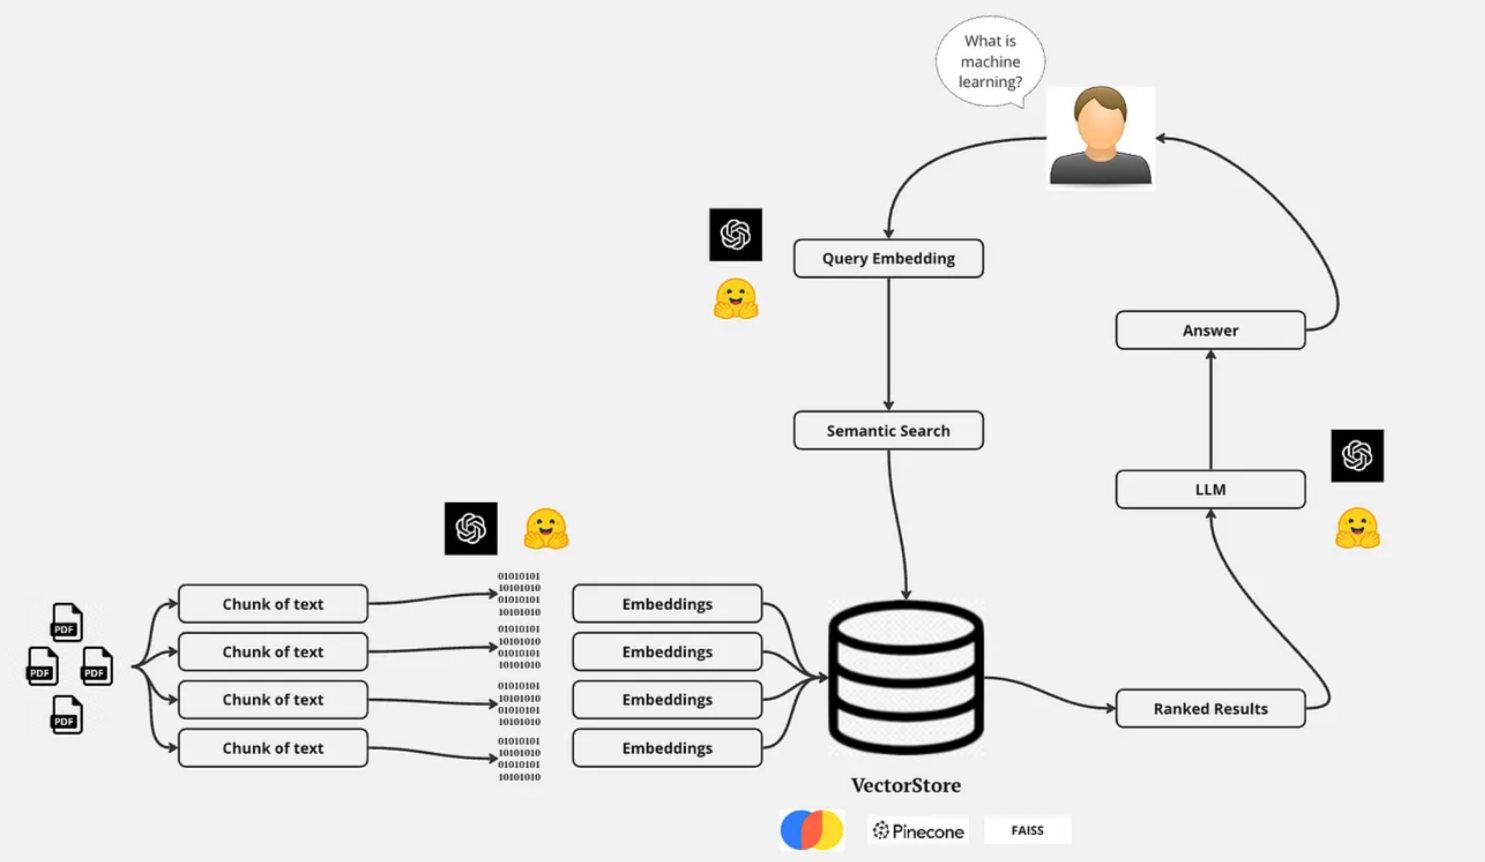
\includegraphics[width=0.9\linewidth]{images/overview}
\end{figure}

Eine gute Illustration stellt das folgende Bild dar:
\newpage
\ \\
\newpage
\section{Question-Answering Projekt}
Das Hauptprojekt ist unter dem Verzeichnis \textbf{NLP Auswertung (lokal)} zu finden.
\\ \\
Der vollständigkeit halber wurde auch einmal der wesentlich einfachere und unkompliziertere Weg hinzugefügt, der sich lediglich auf die OPEN AI stützt und aus dem repository \url{https://github.com/dataprofessor/openai-chatbot/tree/master
} zu entnehmen ist.


\end{document}
